% !TEX TS-program = knitr
\documentclass{article}\usepackage{graphicx, color}
%% maxwidth is the original width if it is less than linewidth
%% otherwise use linewidth (to make sure the graphics do not exceed the margin)
\makeatletter
\def\maxwidth{ %
  \ifdim\Gin@nat@width>\linewidth
    \linewidth
  \else
    \Gin@nat@width
  \fi
}
\makeatother

\IfFileExists{upquote.sty}{\usepackage{upquote}}{}
\definecolor{fgcolor}{rgb}{0.2, 0.2, 0.2}
\newcommand{\hlnumber}[1]{\textcolor[rgb]{0,0,0}{#1}}%
\newcommand{\hlfunctioncall}[1]{\textcolor[rgb]{0.501960784313725,0,0.329411764705882}{\textbf{#1}}}%
\newcommand{\hlstring}[1]{\textcolor[rgb]{0.6,0.6,1}{#1}}%
\newcommand{\hlkeyword}[1]{\textcolor[rgb]{0,0,0}{\textbf{#1}}}%
\newcommand{\hlargument}[1]{\textcolor[rgb]{0.690196078431373,0.250980392156863,0.0196078431372549}{#1}}%
\newcommand{\hlcomment}[1]{\textcolor[rgb]{0.180392156862745,0.6,0.341176470588235}{#1}}%
\newcommand{\hlroxygencomment}[1]{\textcolor[rgb]{0.43921568627451,0.47843137254902,0.701960784313725}{#1}}%
\newcommand{\hlformalargs}[1]{\textcolor[rgb]{0.690196078431373,0.250980392156863,0.0196078431372549}{#1}}%
\newcommand{\hleqformalargs}[1]{\textcolor[rgb]{0.690196078431373,0.250980392156863,0.0196078431372549}{#1}}%
\newcommand{\hlassignement}[1]{\textcolor[rgb]{0,0,0}{\textbf{#1}}}%
\newcommand{\hlpackage}[1]{\textcolor[rgb]{0.588235294117647,0.709803921568627,0.145098039215686}{#1}}%
\newcommand{\hlslot}[1]{\textit{#1}}%
\newcommand{\hlsymbol}[1]{\textcolor[rgb]{0,0,0}{#1}}%
\newcommand{\hlprompt}[1]{\textcolor[rgb]{0.2,0.2,0.2}{#1}}%

\usepackage{framed}
\makeatletter
\newenvironment{kframe}{%
 \def\at@end@of@kframe{}%
 \ifinner\ifhmode%
  \def\at@end@of@kframe{\end{minipage}}%
  \begin{minipage}{\columnwidth}%
 \fi\fi%
 \def\FrameCommand##1{\hskip\@totalleftmargin \hskip-\fboxsep
 \colorbox{shadecolor}{##1}\hskip-\fboxsep
     % There is no \\@totalrightmargin, so:
     \hskip-\linewidth \hskip-\@totalleftmargin \hskip\columnwidth}%
 \MakeFramed {\advance\hsize-\width
   \@totalleftmargin\z@ \linewidth\hsize
   \@setminipage}}%
 {\par\unskip\endMakeFramed%
 \at@end@of@kframe}
\makeatother

\definecolor{shadecolor}{rgb}{.97, .97, .97}
\definecolor{messagecolor}{rgb}{0, 0, 0}
\definecolor{warningcolor}{rgb}{1, 0, 1}
\definecolor{errorcolor}{rgb}{1, 0, 0}
\newenvironment{knitrout}{}{} % an empty environment to be redefined in TeX

\usepackage{alltt}

\usepackage{amsfonts}
\usepackage{amsmath}
\usepackage{amssymb}
\usepackage{amsthm}
\usepackage{caption}
\usepackage{color}
\usepackage{enumerate}
\usepackage{fancyhdr}
\usepackage{hyperref}
\usepackage{graphicx}
\usepackage{latexsym}
\usepackage{listings}
\usepackage{mathrsfs}
\usepackage{natbib}
\usepackage[nottoc]{tocbibind}
\usepackage{url}

\providecommand{\all}{\ \forall \ }
\providecommand{\bs}{\backslash}
\providecommand{\e}{\varepsilon}
\providecommand{\E}{\ \exists \ }
\providecommand{\lm}[2]{\lim_{#1 \rightarrow #2}}
\providecommand{\m}[1]{\mathbb{#1}}
\providecommand{\nv}{{}^{-1}}
\providecommand{\ov}[1]{\overline{#1}}
\providecommand{\p}{\newpage}
\providecommand{\q}{$\quad$ \newline}
\providecommand{\rt}{\rightarrow}
\providecommand{\Rt}{\Rightarrow}
\providecommand{\vc}[1]{\boldsymbol{#1}}
\providecommand{\wh}[1]{\widehat{#1}}

%\renewcommand\bibname{References}
%\renewcommand{\thesection}{Problem \arabic{section}}
%\renewcommand{\thesubsection}{Part \alph{subsection}}
\numberwithin{equation}{section}

\fancyhead{}
\fancyfoot{}
\fancyhead[R]{\thepage}
\fancyhead[C]{Landau}

\hypersetup{
    colorlinks,
    citecolor=black,
    filecolor=black,
    linkcolor=black,
    urlcolor=blue
}

\definecolor{dkgreen}{rgb}{0,0.6,0}
\definecolor{gray}{rgb}{0.5,0.5,0.5}
\definecolor{mauve}{rgb}{0.58,0,0.82}

\lstset{ 
  language=C,                % the language of the code
  basicstyle=\Large,           % the size of the fonts that are used for the code
  numberstyle= \tiny \color{white},  % the style that is used for the line-numbers
  stepnumber=2,                   % the step between two line-numbers. 
  numbersep=5pt,                  % how far the line-numbers are from the code
  backgroundcolor=\color{white},      % choose the background color. You must add \usepackage{color}
  showspaces=false,               % show spaces adding particular underscores
  showstringspaces=false,         % underline spaces within strings
  showtabs=false,                 % show tabs within strings adding particular underscores
  frame=lrb,                   % adds a frame around the code
  rulecolor=\color{black},        % if not set, the frame-color may be changed on line-breaks within not-black text 
  tabsize=2,                      % sets default tabsize to 2 spaces
  captionpos=t,                   % sets the caption-position 
  breaklines=true,                % sets automatic line breaking
  breakatwhitespace=false,        % sets if automatic breaks should only happen at whitespace
  title=\lstname,                   % show the filename of files included with \lstinputlisting;
  keywordstyle=\color{blue},          % keyword style
  commentstyle=\color{gray},       % comment style
  stringstyle=\color{dkgreen},         % string literal style
  escapeinside={\%*}{*)},            % if you want to add LaTeX within your code
  morekeywords={*, ...},               % if you want to add more keywords to the set
  xleftmargin=0.053in, % left horizontal offset of caption box
  xrightmargin=-.03in % right horizontal offset of caption box
}

\DeclareCaptionFont{white}{\color{white}}
\DeclareCaptionFormat{listing}{\parbox{\textwidth}{\colorbox{gray}{\parbox{\textwidth}{#1#2#3}}\vskip-0.05in}}
\captionsetup[lstlisting]{format = listing, labelfont = white, textfont = white}
% For caption-free listings, comment out the 3 lines above and uncomment the 2 lines below.
% \captionsetup{labelformat = empty, labelsep = none}
% \lstset{frame = single}





\begin{document}
\begin{flushleft}
\begin{center} \LARGE
STAT 305 D Homework 9
\end{center}
\begin{center} \Large
Due Apr 11, 2013 at 12:40 PM in class
\end{center}
\large

{\color{red} Show all 6 steps in your hypothesis tests.}



\begin{enumerate}[1. ]

\item  \q
\setkeys{Gin}{width=1\textwidth} 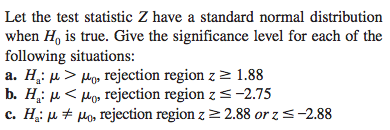
\includegraphics{../../fig/h9p1.png}


\item Use the method of critical values (not p-values) in the following problem. You may assume the test statistic has a N(0,1) distribution. \q
\setkeys{Gin}{width=1\textwidth} 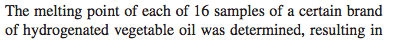
\includegraphics{../../fig/h9p2-1.png}
\setkeys{Gin}{width=1\textwidth} 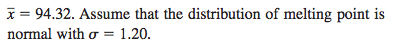
\includegraphics{../../fig/h9p2-2.png}
Do a hypothesis test at significance level $\alpha = 0.01$ to test the hypothesis that the true mean melting point is different from 95.



\item Use the method of critical values (not p-values) in the following problem. \q
\setkeys{Gin}{width=1\textwidth} 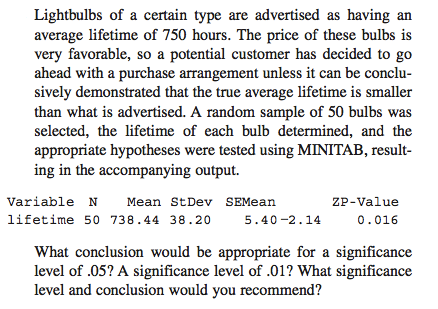
\includegraphics{../../fig/h9p3.png}


\item Use the method of p-values in the following problem. \q
\setkeys{Gin}{width=1\textwidth} 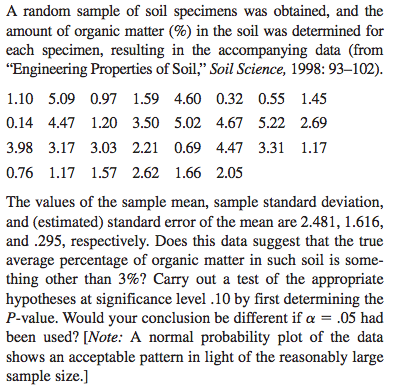
\includegraphics{../../fig/h9p4.png}









\item Vardeman and Jobe chapter 6 section 3 problem 3 (page 385). Solve using the method of p-values at significance level $\alpha = 0.05$.

\setkeys{Gin}{width=1\textwidth} 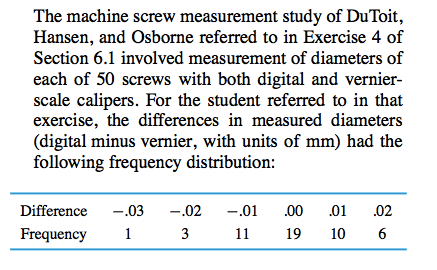
\includegraphics{../../fig/h9p5-1.png}
\setkeys{Gin}{width=1\textwidth} 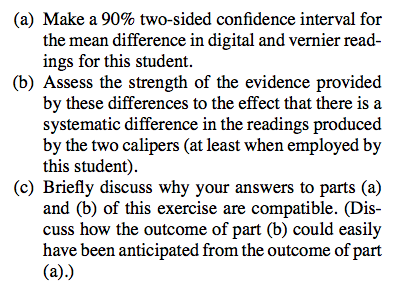
\includegraphics{../../fig/h9p5-2.png}




\item Musculoskeletal neck-and-shoulder disorders are all too common among office staff who perform repetitive tasks using visual display units. The article �Upper-Arm Elevation During Office Work� (Ergonomics, 1996: 1221-1230) reported on a study to determine whether more varied work conditions would have any impact on arm movement. The accompanying data was obtained from a sample of n = 16 subjects. Each observation is the amount of time, expressed as a proportion of total time observed, during which arm elevation was below 30${}^\circ$. The two measurements from each subject were obtained 18 months apart. During this period, work conditions were changed, and subjects were allowed to engage in a wider variety of work tasks. Does the data suggest that true average time during which elevation is below 30� differs after the change from what it was before the change? Do a hypothesis test at $\alpha = 0.1$ to answer this question.

\setkeys{Gin}{width=1\textwidth} 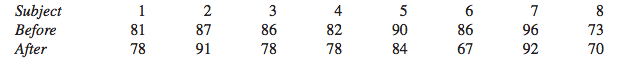
\includegraphics{../../fig/h9p6-1.png}
\setkeys{Gin}{width=1\textwidth} 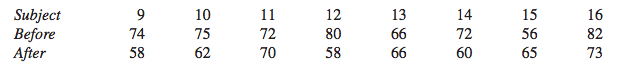
\includegraphics{../../fig/h9p6-2.png}















\item Weekly feedback. You get full credit as long as you write something.
\begin{enumerate}[a. ]
\item Is there any aspect of the subject matter that you currently struggle with? If so, what specifically do you find difficult or confusing? The more detailed you are, the better I can help you.


\item Do you have any questions or concerns about the material, class logistics, or anything else? If so, fire away.

\end{enumerate}
\end{enumerate}
\end{flushleft}
\end{document}
